\problem{Podziały drzew} %B-3

\subproblem %B-3(a)
Niech $T=\langle V,E\rangle$ będzie drzewem binarnym, w~którym $|V|=n\ge2$.
Przez \textbf{krawędź dzielącą} będziemy rozumieć krawędź, po usunięciu której zbiór wierzchołków drzewa $T$ dzieli się na zbiory $A$ i~$B$ takie, że $|A|\le3n/4$ oraz $|B|\le3n/4$.
Udowodnimy przez indukcję względem $n$, że w~każdym takim drzewie istnieje krawędź dzieląca.

Dla $n=2$ twierdzenie zachodzi, ponieważ w~drzewie $T$ istnieje tylko jedna krawędź, po usunięciu której dostajemy zbiory jednoelementowe.
Niech zatem $n>2$ i~załóżmy, że w~drzewie o~$n-1$ wierzchołkach istnieje krawędź dzieląca $e\in E$ taka, że po podziale każdy ze zbiorów $A$ i~$B$ ma co najwyżej $3(n-1)/4$ elementów.
Przyjmijmy bez utraty ogólności, że $|A|\le|B|$, co oznacza, że $|A|\le(n-1)/2$.
Utwórzmy teraz nowe drzewo $T'$, dodając do $V$ nowy wierzchołek $v'$ oraz nową krawędź $\{v',v\}$ do $E$ dla pewnego $v\in V$.
Niech teraz $A'$ oraz $B'$ będą zbiorami wierzchołków w~nowym drzewie utworzonymi w~wyniku podziału krawędzią $e$.
Jeśli $v\in A$, to $A'=A\cup\{v'\}$ oraz $B'=B$.
Oczywiście $|B'|<3n/4$, zbadajmy zatem $A'$:
\[
	|A'| = |A|+1 \le \frac{n-1}{2}+1 = \frac{n+1}{2} \le \frac{3n}{4},
\]
co jest prawdą, o~ile $n\ge2$, zatem w~tym przypadku twierdzenie zachodzi.

Niech teraz $v\in B$.
Stąd $A'=A$ i~$B'=B\cup \{v'\}$, ale z~założenia $|B'|=|B|+1\le(3n+1)/4$, a~zatem $|B'|$ może przekroczyć $3n/4$, co oznacza, że musimy znaleźć inną krawędź dzielącą dla drzewa $T'$ w~przypadku, gdy $|B|=(3n-3)/4$, przy czym $n\ge5$.

Rozważmy drzewo $T'$ przedstawione na rys.\ \ref{fig:B-3a}.
\begin{figure}[ht]
	\centering \includegraphics{fig_b-3.a}
	\caption{Drzewo $T'$ z~drugiego przypadku dowodu.} \label{fig:B-3a}
\end{figure}
Niech $u_1\in B$ oraz $e=\{u_1,u_2\}$.
Oprócz $u_1$ do zbioru $B$ należą wierzchołki ze zbiorów $V_1$ i~$V_2$, a~do zbioru $A$ -- wierzchołek $u_2$ oraz wierzchołki ze zbiorów $V_3$ i~$V_4$.
Załóżmy bez straty ogólności, że $|V_1|\le|V_2|$.
Zbiór $V_2$ jest niepusty, gdyż $|B'|\ge4$, istnieje zatem krawędź $e'=\{u_1,w\}$, gdzie $w\in V_2$.
Pokażemy, że jest to krawędź dzieląca drzewa $T'$.
Rozważmy w~tym celu zbiory $A''$ i~$B''$, na które krawędź $e'$ dzieli zbiór $V\cup\{v'\}$.
Mamy
\[
	|B''| = |V_2| \le |B| = \frac{3n-3}{4} < \frac{3n}{4}
\]
oraz
\[
	|A''| = \bigl|A\cup\{u_1\}\cup V_1\bigr| \le (n-1-|B|)+1+\frac{|B|}{2} = n-\frac{|B|}{2} = \frac{5n+4}{8}.
\]
Skorzystaliśmy z~tego, że $|A|+|B|=n-1$ oraz $|V_1|\le|B|/2$.
Nierówność $|A''|\le3n/4$ zachodzi, o~ile $n\ge4$, więc istotnie $e'$ jest krawędzią dzielącą drzewa $T'$.

Rozpatrzyliśmy wszystkie przypadki, zatem na mocy indukcji twierdzenie zachodzi dla każdego drzewa binarnego $T$.

\subproblem %B-3(b)
Stała $3/4$ jest wystarczająca do dokonywania zrównoważonych podziałów, jak to wykazaliśmy w~punkcie (a).
Przykład drzewa binarnego z~rys.\ \ref{fig:B-3b} pokazuje, że nie można przyjąć na jej miejsce mniejszej wartości.
Usuwając dowolną krawędź tego drzewa, dzielimy zbiór jego wierzchołków na podzbiory, z~których jeden ma trzy elementy.
\begin{figure}[ht]
	\centering 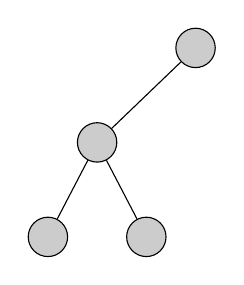
\begin{tikzpicture}[
	level/.style = {level distance=12mm, sibling distance=50mm/2^#1},
	every node/.style = {align=center, inner sep=-1pt, minimum size=5mm, circle, draw, fill=black!20},
]
\node {}
	child {node {}
		child {node {}}
		child {node {}}
	}
	child[missing];
\end{tikzpicture}

	\caption{Drzewo binarne, w~którym najbardziej zrównoważony podział tworzy podzbiór zawierający 3 wierzchołki.} \label{fig:B-3b}
\end{figure}

\subproblem %B-3(c)
Rozważmy następującą procedurę podziału zbioru wierzchołków.
Na początku przyjmujemy, że wynikowe zbiory $A$ i~$B$ są puste.
Usuwając jedną krawędź, możemy podzielić \singledash{$n$}{elementowy} zbiór wierzchołków drzewa na dwa podzbiory, z~których większy będzie składać się z~co najwyżej $3n/4$ wierzchołków, co wynika na podstawie punktu (a).
Mniejszy podzbiór sumujemy z~jednym ze zbiorów wynikowych, natomiast większy z~nich będzie podlegał dalszemu podziałowi.
Podczas działania procedury pilnujemy, aby rozmiary zbiorów $A$ i~$B$ nie przekroczyły $\lceil n/2\rceil$.
Procedurę podziału zakończymy w~momencie, gdy jeden z~tych zbiorów będzie zawierał $\lceil n/2\rceil$ elementów, gdyż drugi zbiór zawiera wtedy $\lfloor n/2\rfloor$ elementów.

Zauważmy, że maksymalną liczbę podziałów dla zadanego drzewa wykonamy w~przypadku, gdy po każdym kroku zostanie do podziału zbiór o~rozmiarze $3/4$ rozmiaru zbioru z~poprzedniego kroku.
Niech $k$ będzie taką maksymalną liczbą podziałów drzewa o~$n$ wierzchołkach.
Zachodzi wtedy $(3/4)^kn=1$, ponieważ zbioru jednoelementowego nie trzeba już dalej dzielić.
Stąd mamy $k=\log_{4/3}n$, a~zatem należy usunąć co najwyżej $k=O(\lg n)$ krawędzi.
